\documentclass[border=10pt]{standalone}

\usepackage{tikz}
\usepackage{tikzsymbols}
\usetikzlibrary{calc,patterns,shapes.geometric}

\def\centerarc[#1](#2)(#3:#4:#5){\draw[#1] ($(#2)+({#5*cos(#3)},{#5*sin(#3)})$) arc (#3:#4:#5);}

\begin{document}
	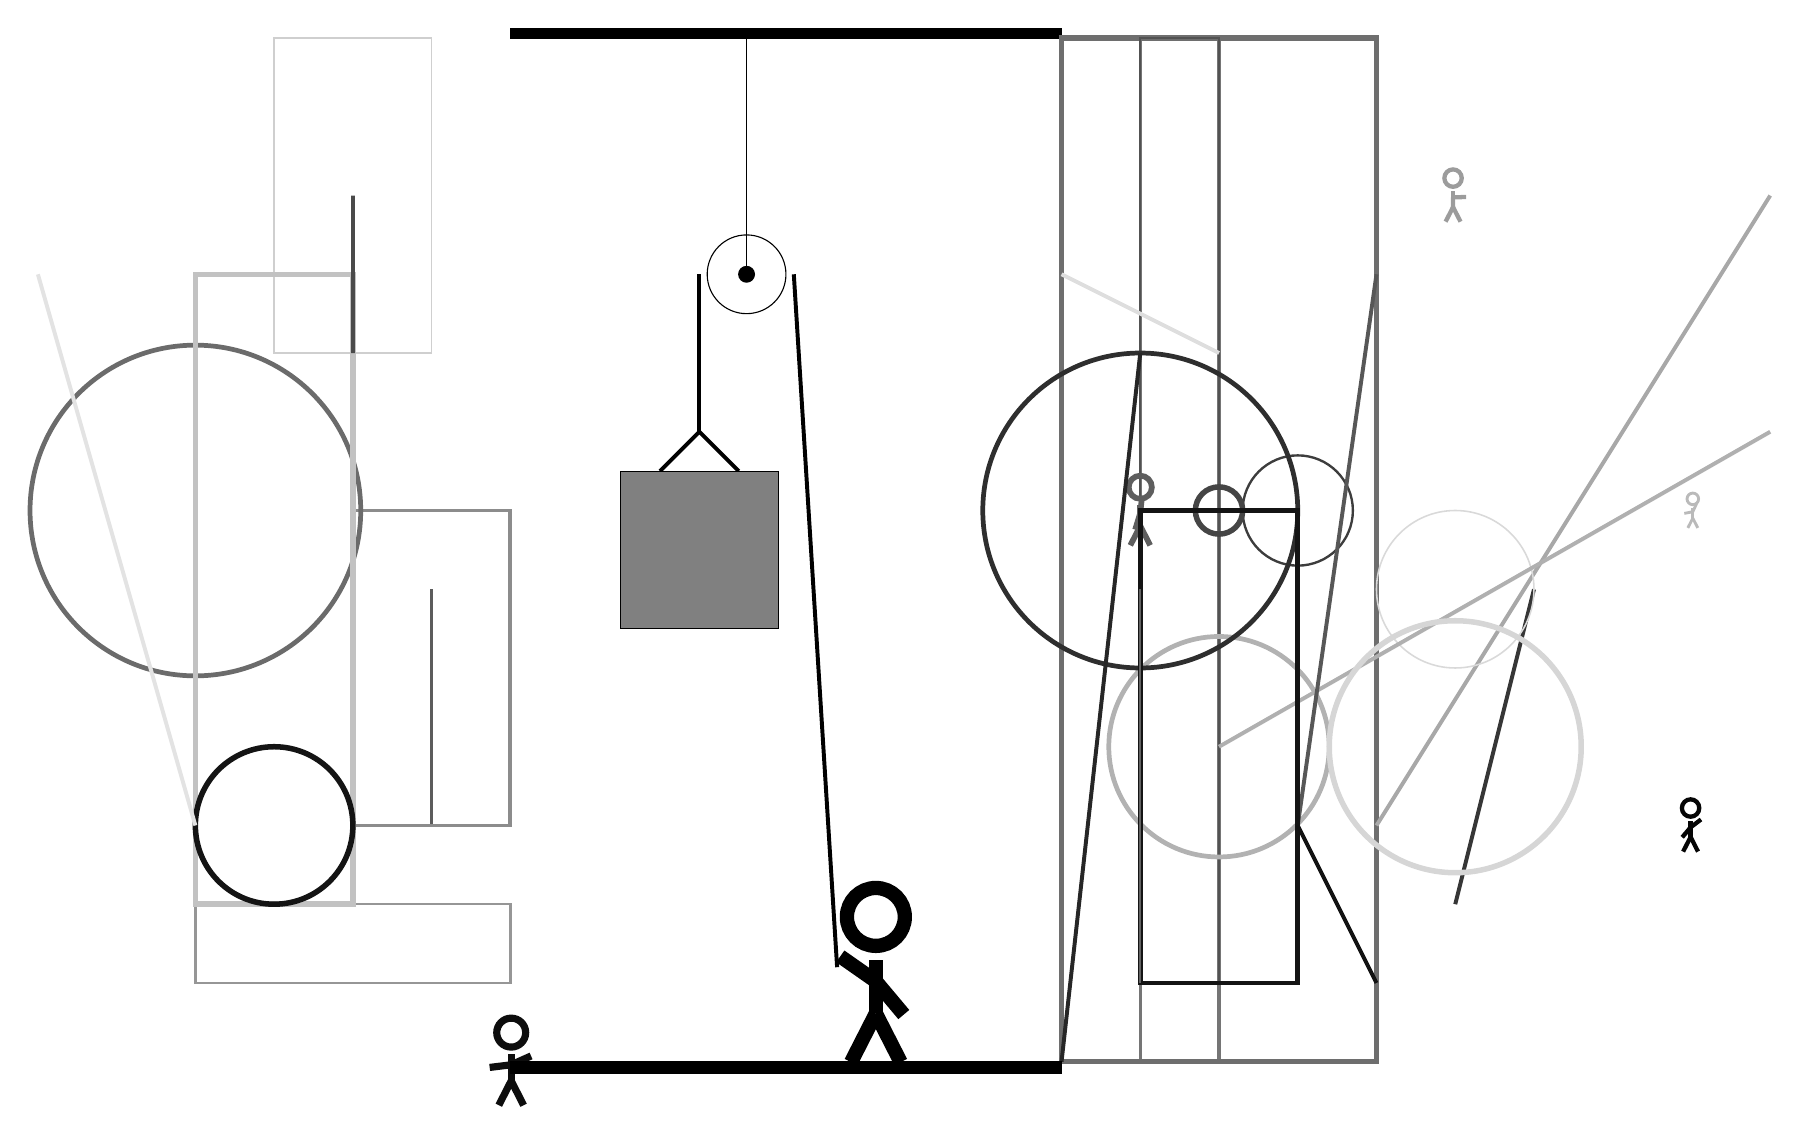
\begin{tikzpicture}
		%%%%% START %%%%%
		
		\draw[fill=black] (-2, 10) rectangle (5, 10.125);
		
		\draw (1, 7) circle (0.5);
		\draw[fill=black] (1, 7) circle (0.1);
		\draw (1, 10) -- (1, 7);
		
		\draw [line width=0.3mm, color=black!76](8, 4) circle (0.7);
		
		\draw[line width=0.3mm, color=black!41] (-2, -2) rectangle (-6, -1);
		\draw[line width=0.3mm, color=black!64] (-3, 3) rectangle (-3, 0);
		\draw[line width=0.5mm, color=black!45] (-2, 0) rectangle (-4, 4);
		\draw[line width=0.4mm, color=black!54] (7, -3) rectangle (6, 10);
		
		\draw[line width=0.5mm, color=black!79](10, -1) -- (11, 3);
		
		\draw[line width=0.7mm, color=black!57] (5, -3) rectangle (9, 10);
		\draw [line width=0.6mm, color=black!58](-6, 4) circle (2.1);
		\draw[line width=0.3mm, color=black!68] (7, 10) rectangle (6, -2);
		
		\node[line width=0.6mm, color=black!39] at (10, 8) {\Strichmaxerl[3][89][2]};
		
		\node[line width=0.6mm, color=black!98] at (13, 0) {\Strichmaxerl[3][50][37]};
		\draw [line width=0.6mm, color=black!30](7, 1) circle (1.4);
		\node[line width=0.4mm, color=black!95] at (-2, -3) {\Strichmaxerl[5][7][24]};
		
		\draw [line width=0.7mm, color=black!73](7, 4) circle (0.3);
		\draw[line width=0.5mm, color=black!13](7, 6) -- (5, 7);
		\node[line width=0.2mm, color=black!27] at (13, 4) {\Strichmaxerl[2][11][65]};
		
		\draw[line width=0.5mm, color=black!34](9, 0) -- (14, 8);
		
		\draw [line width=0.2mm, color=black!15](10, 3) circle (1.0);
		\draw[line width=0.2mm, color=black!19] (-3, 6) rectangle (-5, 10);
		\draw[line width=0.7mm, color=black!24] (-4, -1) rectangle (-6, 7);
		\draw[line width=0.5mm, color=black!31](7, 1) -- (14, 5);
		
		\draw[line width=0.5mm, color=black!66](9, 7) -- (8, 0);
		\draw [line width=0.7mm, color=black!92](-5, 0) circle (1.0);
		\draw [line width=0.6mm, color=black!82](6, 4) circle (2.0);
		\node[line width=0.5mm, color=black!63] at (6, 4) {\Strichmaxerl[4][73][84]};
		
		\draw[line width=0.3mm, color=black!43] (-4, -3) rectangle (-4, -3);
		\draw[line width=0.6mm, color=black!92] (6, -2) rectangle (8, 4);
		\draw[line width=0.6mm, color=black!71] (-4, 6) rectangle (-4, 8);
		\draw [line width=0.7mm, color=black!16](10, 1) circle (1.6);
		\draw[line width=0.5mm, color=black!93](9, -2) -- (8, 0);
		\draw[line width=0.5mm, color=black!85](6, 6) -- (5, -3);
		
		\draw[line width=0.5mm, color=black!11](-6, 0) -- (-8, 7);
		\draw[line width=0.2mm, color=black!61] (6, -2) rectangle (6, 3);
		
		\draw[line width=0.5mm] (-0.1, 4.5) -- (0.4, 5.0) -- (0.9, 4.5);
		\draw[fill=black!50] (-0.6, 4.5) rectangle (1.4, 2.5);
		
		\draw[line width=0.5mm] (0.4, 7) -- (0.4, 5.0);
		\centerarc[line width=0.5mm](1, 7)(0:180:0.6);
		\draw[line width=0.5mm](1.6, 7) -- (2.15, -1.8);
		
		\node at (2.6, -1.9) {\Strichmaxerl[10][-35][-50]};
		
		\draw[fill=black] (-2, -3) rectangle (5, -3.15);
		
		%%%%% END %%%%%
	\end{tikzpicture}
\end{document}